\documentclass{article}

% Language setting
% Replace `english' with e.g. `spanish' to change the document language
\usepackage[english]{babel}

% Set page size and margins
% Replace `letterpaper' with `a4paper' for UK/EU standard size
\usepackage[letterpaper,top=2cm,bottom=2cm,left=3cm,right=3cm,marginparwidth=1.75cm]{geometry}

% Useful packages
\usepackage{amsmath}
\usepackage{graphicx}
\usepackage[colorlinks=true, allcolors=blue]{hyperref}
\usepackage{tikz}
\usetikzlibrary{positioning, arrows.meta, shapes.geometric}

\title{Smart Visual Alarm System for House Monitoring using Tiny CNN Models and MQTT}
\author{Stefano Murtas}

\begin{document}
\maketitle

\begin{abstract}
Your abstract.
\end{abstract}

\section{Introduction}

The Internet of Things (IoT) enables the development of distributed systems where embedded devices can sense the environment, process data locally, and communicate relevant events to remote users or services. In recent years, the integration of machine learning techniques into IoT devices has made it possible to move part of the intelligence directly to the edge, reducing latency, bandwidth usage, and dependence on cloud services.

This project focuses on the design and implementation of a smart visual alarm system for monitoring a mountain house environment. The selected scenario is motivated by a real use case: people and animals may pass near the house, including during the night, and an automatic notification system could be useful to detect relevant events. Instead of implementing a generic people detection system, the goal is to classify the observed scene into a small set of classes: empty scene, person, and generic animal.

The proposed system is based on an ESP32-S3-EYE camera board and a Raspberry Pi used as an IoT gateway. The ESP32-S3-EYE, shown in Figure~\ref{fig:esp32_s3_eye},  acquires visual information from the monitored area and performs visual classification using lightweight neural network models. When a relevant event is detected, the device publishes an MQTT message containing information such as the predicted class, confidence score, timestamp, and event identifier. The Raspberry Pi receives the event through an MQTT broker, logs the information, and forwards an alert to the user through a Telegram bot.

A central part of the project is the evaluation of lightweight neural network architectures suitable for resource-constrained visual recognition tasks. In particular, three models are considered: a small convolutional baseline model, MCUNet, and TinyViT. These models are trained and evaluated on a dataset collected in the target environment, with the aim of comparing their classification performance and efficiency. The comparison considers both machine learning metrics, such as accuracy, precision, recall, F1-score, and confusion matrix, and system-oriented metrics, such as model size and inference latency.

The final objective is to obtain a working prototype that combines embedded vision, lightweight machine learning, MQTT communication, and remote notification. The project also aims to evaluate the practical limitations of deploying visual intelligence in a real IoT scenario, especially under varying illumination conditions and with a limited number of training samples.

\section{System Overview}

\subsection{Use Case and Target Scenario}

The target scenario of this project is the monitoring of a mountain house environment. In this context, people and animals may pass near the entrance or in the surrounding outdoor area, also during evening or night hours. The objective is to develop a smart visual alarm system able to detect relevant visual events and notify the user remotely.

Unlike a generic indoor people detection system, this project focuses on a more specific real-world scenario. The monitored area is expected to contain different types of situations: an empty scene, the presence of a person, or the presence of a generic animal. The goal is not to recognize the animal species, since this would require a larger and more complex dataset, but to distinguish between the main classes that are relevant for the alarm system.

The camera is intended to be positioned near the entrance of the house or in a protected point with a clear view of the monitored area. Since an automatic light is already installed and turns on when motion is detected, the system can also be tested in low-light conditions without requiring an additional infrared camera. This makes the scenario more realistic while keeping the hardware setup simple.

The proposed use case is therefore based on three target classes:
\begin{itemize}
    \item \textbf{Empty}: no relevant subject is visible in the monitored area;
    \item \textbf{Person}: at least one person is visible in the scene;
    \item \textbf{Animal}: at least one generic animal is visible in the scene.
\end{itemize}

When the system detects a relevant class, namely \textit{person} or \textit{animal}, it generates an alarm event. The event is then transmitted through MQTT to the Raspberry Pi backend, which logs the event and sends a notification to the user through Telegram. This use case allows the evaluation of both the visual classification performance and the reliability of the IoT notification pipeline in a realistic environment.

\subsection{General System Architecture}

The proposed system is composed of an ESP32-S3-EYE camera node, a Raspberry Pi gateway, an MQTT communication layer, and a Telegram notification service. The ESP32-S3-EYE is responsible for acquiring images from the monitored area and performing visual classification. When a relevant event is detected, the device publishes an MQTT message containing the predicted label, the confidence score, the timestamp, and an event identifier.

The Raspberry Pi acts as the IoT gateway of the system. It runs the MQTT broker and a Python backend that subscribes to the alarm topic, stores the received events, and forwards notifications to the user through a Telegram bot. This architecture separates the visual sensing and classification task from the backend communication and logging functionalities.

\begin{figure}[h]
\centering
\resizebox{0.85\textwidth}{!}{
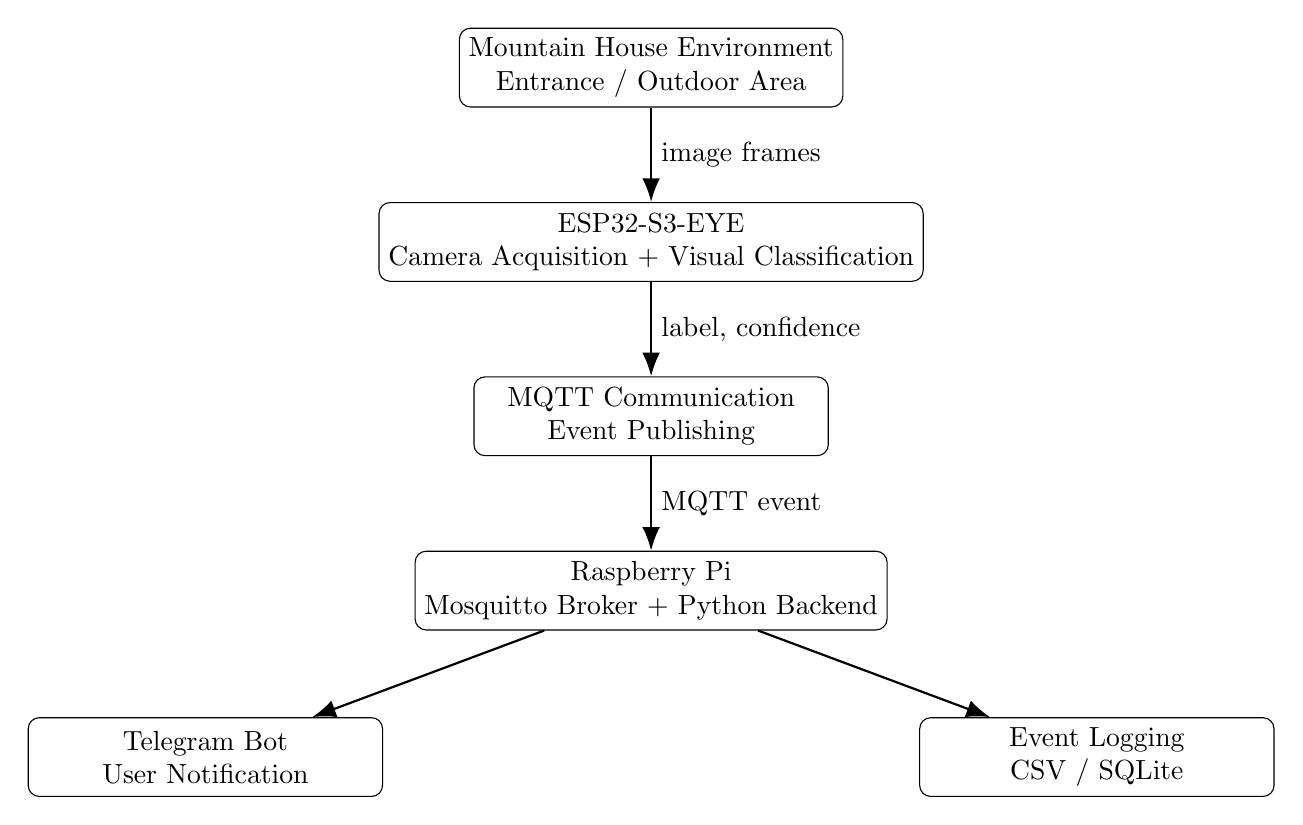
\begin{tikzpicture}[
    node distance=1.2cm,
    block/.style={
        rectangle,
        rounded corners,
        draw,
        align=center,
        minimum width=4.5cm,
        minimum height=1cm
    },
    arrow/.style={
        -{Latex[length=3mm]},
        thick
    }
]

\node[block] (scene) {Mountain House Environment\\Entrance / Outdoor Area};

\node[block, below=of scene] (esp32) {ESP32-S3-EYE\\Camera Acquisition + Visual Classification};

\node[block, below=of esp32] (mqtt) {MQTT Communication\\Event Publishing};

\node[block, below=of mqtt] (raspberry) {Raspberry Pi\\Mosquitto Broker + Python Backend};

\node[block, below left=1.1cm and 0.4cm of raspberry] (telegram) {Telegram Bot\\User Notification};

\node[block, below right=1.1cm and 0.4cm of raspberry] (log) {Event Logging\\CSV / SQLite};

\draw[arrow] (scene) -- node[right] {image frames} (esp32);
\draw[arrow] (esp32) -- node[right] {label, confidence} (mqtt);
\draw[arrow] (mqtt) -- node[right] {MQTT event} (raspberry);
\draw[arrow] (raspberry) -- (telegram);
\draw[arrow] (raspberry) -- (log);

\end{tikzpicture}
}
\caption{General architecture of the proposed smart visual alarm system.}
\label{fig:system_architecture}
\end{figure}

\begin{figure}
\centering
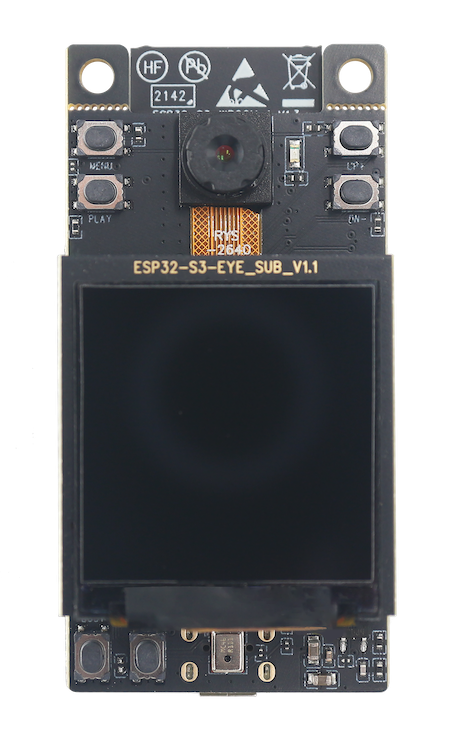
\includegraphics[width=0.25\linewidth]{ESP32-S3-EYE-isometric.png}
\caption{\label{fig:esp32_s3_eye}ESP32-S3-EYE board used for image acquisition and visual classification in the proposed smart visual alarm system.}
\end{figure}

\section{GitHub Repository}

You can find the whole project at \url{https://github.com/smurtas/Smart-Visual-Alarm-System.git}.

\bibliographystyle{alpha}
\bibliography{sample}

\end{document}
